% fig1_overview.tex -- Figure 1 (figure*, 7.0 in): the tool as a schematic (left) and the headline result (right).
%
% Use inside a figure* (main.tex):   \begin{figure*}% fig1_overview.tex -- Figure 1 (figure*, 7.0 in): the tool as a schematic (left) and the headline result (right).
%
% Use inside a figure* (main.tex):   \begin{figure*}% fig1_overview.tex -- Figure 1 (figure*, 7.0 in): the tool as a schematic (left) and the headline result (right).
%
% Use inside a figure* (main.tex):   \begin{figure*}% fig1_overview.tex -- Figure 1 (figure*, 7.0 in): the tool as a schematic (left) and the headline result (right).
%
% Use inside a figure* (main.tex):   \begin{figure*}\input{figures/fig1_overview}\caption{...}\label{fig:overview}\end{figure*}
% Needs: smpreprint.sty (any option; colors sm*, \smfigfont), TikZ libraries arrows.meta, positioning, calc,
%        shadows (loaded by smpreprint.sty), graphicx, and \graphicspath containing figures/ (main.tex) or the
%        current directory (figures/fig1_standalone.tex).
% Right part: fig1_headline.pdf, generated from data by scripts/fig_headline.py (never edited by hand). If it is
%        missing the figure shows a marked frame instead, so the paper still builds.
%
% Schematic contents and where each item comes from (CE = ../citation-equity, read only):
%   draft sheet, the flagged heading "Why espresso turns bitter"  src: CE/samples/espresso-bitterness/before.md line 11
%   stage 1, eleven checks, each graded                           src: CE/docs/evidence.md line 3 (eleven checks), CE c908431
%     pip colors in check order (section headings of CE/docs/evidence.md at CE c908431): standalone-paragraphs untested (l.90),
%     question-headings mixed (l.103), lists mixed (l.119), statistics mixed (l.133), tables untested (l.148), expert-quotes
%     mixed (l.162), cited-sources mixed (l.178), direct-answer-lead mixed (l.193), question-coverage mixed (l.208),
%     comparisons mixed (l.225), reader-words mixed (l.241); "No check is graded strong or moderate today" (l.34)
%   "a writing checklist, not a forecast"                         src: CE/apps/workspace/components/draft/score-card.tsx
%                                                                  line 112 and CE/README.md line 32 (CE c908431)
%   stage 3 label "Test the advice"; the bubble "[1] [2]" stands for numbered citations in an answer (illustrative)
%   stage 2, the card: an edit suggestion the engine emits on the espresso before draft (checkId question-headings,
%     kind edit, title 'End this heading with "?", or reword it as a question'; the check is shown as Not scored since E3, CE c908431)
%                                                                  src: `ce analyze CE/samples/espresso-bitterness/before.md --json`
%                                                                  at CE commit c908431 (rechecked; data/scores.json records the
%                                                                  commit). Question headings is now an unscored note (weight 0):
%                                                                  the card still shows how a ready edit works.
%   Apply / Undo, applied only if the anchored text is unchanged, no bulk action
%                                                                  src: CE/README.md line 13; CE/docs/architecture.md line 81
%   stage 3, draft + competitor pages, BM25 top 8, local model, 8 seeded runs per question, retrieved / cited / share
%     against chance                                               src: CE/samples/README.md line 39; CE/docs/architecture.md lines 52 to 55
%   bottom strip, site readiness: 7 items in CE/docs/evidence.md order (section headings at CE c908431), byline untested (l.275),
%     dates mixed (l.287), structured data mixed (l.299), indexing directives strong (l.313), canonical untested (l.326),
%     crawler access strong (l.336), renders without JavaScript moderate (l.370)
%   who gets cited: answers the author pastes, or the optional live check   src: CE/docs/evidence.md line 387; CE/README.md line 15
%   "never changes the score"                                     src: CE/docs/evidence.md line 262
%   lock: drafts stay on your machine                             src: CE/README.md line 68
%
% Draft caption (the caption lives in main.tex; numbers there come from numbers.tex, not typed):
%   \caption{\figtakeaway{Following the tool's suggestions raises its checklist score by 26 to 29 points, but
%   raises citation share on four open models by only 1 to 3 points.} Left: Citation Equity checks a draft against
%   eleven checks, each shown with the grade of its evidence (1); suggests span-anchored fixes that the author applies
%   one at a time (2); and tests the draft against competitor pages on a local model (3). Site readiness and who
%   gets cited are reported apart and never change the score. \panel{a} Checklist score of the two sample drafts
%   before and after the suggestions (foundation preset, \keyring{smBefore} before, \keyring{smAfter} after; the
%   rise is built in, since the suggestions target the checks). \panel{b} Citation share of the target page in the
%   pre-registered harness on four open models (n = 8 questions x 8 seeds, synthetic packs, target always among the
%   8 sources), one line per model with its relative change, faint lines per sample draft; the after-minus-before
%   contrast is exploratory. Dotted: chance (1 of 8 sources); dashed: the off-topic control. Score marks are hollow
%   and citation marks filled, so the two are never read as one quantity.}
%   [src for the caption's numbers: data/scores.json; CE/experiments/results/sensitivity/sensitivity_*.json]
%
\begingroup
\smfigfont\fontsize{5.5}{6.5}\selectfont
\begin{tikzpicture}[x=1cm, y=1cm, line cap=round, line join=round,
  >={Stealth[length=3.2pt, width=3pt]},
  smpanel/.style={fill=smTint, draw=none, rounded corners=3pt},
  smcard/.style={fill=white, draw=smPaperRule, line width=0.5pt, rounded corners=2.5pt},
  smstage/.style={font=\smfigfont\fontseries{sb}\selectfont\fontsize{7.4}{9}\selectfont, text=smInk, anchor=west,
    inner sep=0pt},
  smnum/.style={circle, fill=smAfter, text=white, inner sep=0pt, minimum size=8.6pt,
    font=\smfigfont\bfseries\fontsize{5.8}{6}\selectfont},
  smsoft/.style={text=smInkSoft, inner sep=0pt},
  smink/.style={text=smInk, inner sep=0pt},
  smnote/.style={text=smInkSoft, inner sep=0pt, font=\smfigfont\itshape\fontsize{5.5}{6.4}\selectfont},
  smhead/.style={text=smInk, inner sep=0pt, font=\smfigfont\fontseries{sb}\selectfont\fontsize{6.2}{7}\selectfont},
  smflow/.style={->, draw=smAfter, line width=0.8pt},
  smthin/.style={->, draw=smInkSoft, line width=0.5pt, >={Stealth[length=2.4pt, width=2.4pt]}},
  smpip/.style={rounded corners=0.8pt, draw=none},
  smbox/.style={fill=white, draw=smRule, line width=0.45pt, rounded corners=2pt, inner xsep=3pt, inner ysep=1.8pt,
    text=smInk},
  smchip/.style={rounded corners=2pt, inner xsep=2pt, inner ysep=1.2pt, font=\smfigfont\fontsize{5.3}{6}\selectfont},
]
% ------------------------------------------------------------------------------------------------- helpers
% \smpip{x}{y}{options}: one grade pip (a small rounded square)
\def\smpip#1#2#3{\fill[smpip, #3] (#1-0.075, #2-0.075) rectangle (#1+0.075, #2+0.075);}
% \smdoc{x}{y}{fill}{draw}: a page glyph with a folded corner
\def\smdoc#1#2#3#4{%
  \filldraw[fill=#3, draw=#4, line width=0.45pt, rounded corners=0.3pt]
    (#1-0.085,#2-0.115) -- (#1+0.085,#2-0.115) -- (#1+0.085,#2+0.06) -- (#1+0.03,#2+0.115) -- (#1-0.085,#2+0.115) -- cycle;}

% Geometry (cm): the schematic spans x 0 to 10.3; the headline panel (7.24 cm = 2.85 in) is right-aligned at 17.78
% (= 7.0 in); main row y 1.42 to 4.85; the bottom strip y 0.05 to 1.2; stage headers at y 5.17.
% columns: draft 0.05-1.95 | stage 1: 2.2-4.4 | stage 2: 4.65-7.45 | stage 3: 7.7-10.3

% ================================================================================================= left: schematic
% ---- stage headers
\node[smstage] at (0.05, 5.17) {Your draft};
\node[smnum] (n1) at (2.32, 5.17) {1};
\node[smstage, right=3pt of n1] {Check};
\node[smnum] (n2) at (4.77, 5.17) {2};
\node[smstage, right=3pt of n2] {Suggest, never rewrite};
\node[smnum] (n3) at (7.86, 5.17) {3};
\node[smstage, right=3pt of n3] {Test the advice};

% ---- the draft sheet
\filldraw[fill=smPaper, draw=smPaperRule, line width=0.5pt, rounded corners=2.5pt,
  drop shadow={opacity=0.10, shadow xshift=0.5pt, shadow yshift=-0.7pt}] (0.05,1.42) rectangle (1.95,4.85);
\begin{scope}[line width=1.4pt, smRule!75]
  \draw[smInk!70, line width=2.0pt] (0.22,4.6) -- (1.45,4.6);          % title
  \foreach \y/\l in {4.36/1.76, 4.23/1.68, 4.10/1.78, 3.97/1.20} \draw (0.22,\y) -- (\l,\y);
  \foreach \y/\l in {3.16/1.78, 3.03/1.70, 2.90/1.80, 2.77/1.58, 2.64/1.76, 2.51/1.05} \draw (0.22,\y) -- (\l,\y);
  \foreach \y/\l in {2.02/1.74, 1.89/1.66, 1.76/1.20} \draw (0.22,\y) -- (\l,\y);
\end{scope}
% the flagged heading, anchored: brand-soft fill and the dotted mark underline
\node[anchor=west, inner xsep=1.5pt, inner ysep=1.1pt, fill=smBrandSoft, rounded corners=1pt, text=smInk, align=left,
  font=\smfigfont\fontseries{sb}\selectfont\fontsize{5.6}{6.4}\selectfont] (span) at (0.16,3.55) {Why espresso\\turns bitter};
\draw[smMark, line width=0.75pt, dash pattern=on 0.6pt off 1.1pt]
  ($(span.south west)+(1.5pt,0.5pt)$) -- ($(span.south east)+(-1.5pt,0.5pt)$);
\draw[smInk!55, line width=1.6pt] (0.22,2.3) -- (1.0,2.3);              % a second, plain heading

% ---- lock: nothing leaves the machine
\filldraw[fill=white, draw=smRule, line width=0.45pt, rounded corners=2.5pt] (0.05,0.05) rectangle (1.95,1.2);
\begin{scope}[shift={(0.31,0.6)}]
  \draw[smAfter, line width=0.95pt] (-0.08,0.02) -- (-0.08,0.11) arc[start angle=180, end angle=0, radius=0.08] -- (0.08,0.02);
  \fill[smAfter, rounded corners=0.8pt] (-0.125,-0.16) rectangle (0.125,0.04);
  \fill[white] (0,-0.06) circle (0.026);
\end{scope}
\node[anchor=west, smink, align=left] at (0.52,0.62)
  {{\fontseries{sb}\selectfont Stays on your}\\{\fontseries{sb}\selectfont machine:} static\\site, no server};

% ---- flow arrows between the stages
\draw[smflow] (1.98,3.8) -- (2.18,3.8);
\draw[smflow] (4.42,3.8) -- (4.63,3.8);
\draw[smflow] (7.47,3.8) -- (7.68,3.8);

% ---- stage 1: check
\fill[smpanel] (2.2,1.42) rectangle (4.4,4.85);
\begin{scope}[shift={(3.3,3.86)}]
  \draw[white, line width=3.4pt] (180:0.58) arc[start angle=180, end angle=0, radius=0.58];
  \draw[smAfter, line width=3.4pt] (180:0.58) arc[start angle=180, end angle=55, radius=0.58];
  \node[smhead] at (0,0.16) {score};
  \node[smsoft, font=\smfigfont\fontsize{5.1}{6}\selectfont] at (0,-0.03) {0 to 100};
\end{scope}
% label matches the score card of the tool at CE c908431 (CE/apps/workspace/components/draft/score-card.tsx line 112,
% "A writing checklist, not a forecast."), as Figure 2 and Section 2.1 say
\node[smnote, align=center] at (3.3,3.42) {a writing checklist,\\ not a forecast};
\node[smink, align=center] at (3.3,2.86) {eleven checks, each shown\\ with its evidence grade};
% pips in check order (grades: CE/docs/evidence.md, see the header); eleven pips centred on the panel (x 3.3)
\foreach \i/\g in {0/smUntested, 1/smMixed, 2/smMixed, 3/smMixed, 4/smUntested, 5/smMixed, 6/smMixed,
                   7/smMixed, 8/smMixed, 9/smMixed, 10/smMixed} {\smpip{2.425+0.175*\i}{2.43}{fill=\g}}
\smpip{2.5}{2.07}{fill=smMixed}    \node[smsoft, anchor=west] at (2.61,2.07) {mixed};
\smpip{3.3}{2.07}{fill=smUntested} \node[smsoft, anchor=west] at (3.41,2.07) {untested};
\node[smnote] at (3.3,1.68) {none strong or moderate};

% ---- stage 2: suggest, never rewrite
\fill[smpanel] (4.65,1.42) rectangle (7.45,4.85);
\filldraw[smcard] (4.78,2.47) rectangle (7.32,4.72);
\node[smchip, fill=smTint, text=smInkSoft, anchor=west] (chk) at (4.86,4.5) {question headings};
\node[smchip, fill=smTint, text=smInkSoft, right=2pt of chk] {not scored};
\node[anchor=north west, smhead] at (4.88,4.27) {End this heading with ``?''};
\node[anchor=west, smsoft, font=\smfigfont\bfseries\fontsize{6}{6}\selectfont, text=smBefore] at (4.88,3.84) {\textminus};
\node[anchor=west, text=smBefore!80!black, inner sep=0pt] at (5.05,3.84) {Why espresso turns bitter};
\node[anchor=west, smsoft, font=\smfigfont\bfseries\fontsize{6}{6}\selectfont, text=smAfter] at (4.88,3.56) {+};
\node[anchor=west, text=smAfter, inner sep=0pt] at (5.05,3.56)
  {Why espresso turns bitter\setlength{\fboxsep}{0.6pt}\colorbox{smBrandSoft}{\fontseries{b}\selectfont ?}};
\node[smnote, anchor=west] at (4.88,3.25) {anchored to the exact words};
\node[smchip, fill=smAfter, text=white, anchor=west, font=\smfigfont\fontseries{sb}\selectfont\fontsize{5.8}{6.5}\selectfont,
  inner xsep=4pt, inner ysep=2pt] (apply) at (4.88,2.9) {Apply};
\node[anchor=west, smsoft, right=6pt of apply] (undo) {Undo};
\node[anchor=west, smsoft, right=6pt of undo] {Skip};
\node[anchor=west, text=smOfftopic, inner sep=0pt] (all) at (4.9,2.13) {Apply all};
\draw[smInkSoft, line width=0.6pt] ($(all.west)+(-1pt,0)$) -- ($(all.east)+(1pt,0)$);
\node[anchor=west, smsoft, right=5pt of all] {no bulk action};
\node[smnote, align=center] at (6.05,1.7) {applies only while the anchored\\ text is unchanged};

% ---- stage 3: test the advice
\fill[smpanel] (7.7,1.42) rectangle (10.3,4.85);
\smdoc{8.17}{4.55}{smAfter}{smAfter}
\foreach \i in {1,...,7} {\smdoc{8.17+0.235*\i}{4.55}{white}{smBefore}}
\node[smsoft, anchor=north] (pages) at (9.0,4.37) {your draft + competitor pages};
\node[smbox, below=7pt of pages] (bm) {BM25 retrieval, top 8};
\node[smbox, below=6pt of bm] (lm) {open model, run locally};
\node[smink, below=6pt of lm] (runs) {8 seeded runs per question};
\draw[smthin] (pages.south) -- (bm.north);
\draw[smthin] (bm.south) -- (lm.north);
\draw[smthin] (lm.south) -- (runs.north);
\foreach \k/\t in {0/{retrieved?}, 1/{cited?}, 2/{share against chance}} {
  \fill[smAfter] (8.33,{2.46-0.24*\k}) circle (0.038);
  \node[anchor=west, smink] at (8.43,{2.46-0.24*\k}) {\t};
}
\node[smnote] at (9.0,1.66) {before vs.\ after, paired test};

% ---- bottom strip: beyond the draft
\draw[smRule, line width=0.5pt, dash pattern=on 2pt off 1.5pt, rounded corners=3pt] (2.2,0.05) rectangle (10.3,1.2);
\node[fill=white, inner xsep=3pt, inner ysep=1pt, anchor=west, text=smInkSoft,
  font=\smfigfont\fontseries{sb}\selectfont\fontsize{5.8}{7}\selectfont] at (2.32,1.2)
  {Beyond the draft: reported apart, never changes the score};
% site readiness
\node[anchor=west, smhead] (sr) at (2.36,0.86) {Site readiness};
\node[smsoft, anchor=west, right=4pt of sr] {can engines reach the page?};
\foreach \i/\g in {0/smUntested, 1/smMixed, 2/smMixed, 3/smStrong, 4/smUntested, 5/smStrong, 6/smModerate}
  {\smpip{2.44+0.194*\i}{0.53}{fill=\g}}
\node[anchor=west, inner sep=0pt, text=smStrong] at (3.86,0.53)
  {\fontseries{sb}\selectfont strong:\fontseries{m}\selectfont\ crawler access, indexing};
\node[smnote, anchor=west] at (2.36,0.25) {seven items, graded on operator documentation};
% who gets cited
\draw[smRule, line width=0.4pt] (6.6,0.18) -- (6.6,1.0);
\node[anchor=west, smhead] at (6.75,0.86) {Who gets cited};
\node[smsoft, anchor=west, align=left] at (6.75,0.42) {AI answers you paste in,\\ or an optional live check};
\begin{scope}[shift={(9.75,0.62)}]
  \filldraw[fill=white, draw=smInkSoft, line width=0.45pt, rounded corners=2pt] (-0.34,-0.18) rectangle (0.34,0.18);
  \fill[white] (-0.15,-0.175) -- (-0.05,-0.175) -- (-0.17,-0.3) -- cycle;
  \draw[smInkSoft, line width=0.45pt] (-0.15,-0.18) -- (-0.17,-0.3) -- (-0.05,-0.18);
  \node[font=\smfigfont\fontseries{sb}\selectfont\fontsize{5.4}{6}\selectfont, text=smAfter, inner sep=0pt] at (0,0) {[1] [2]};
\end{scope}

% ================================================================================================= right: headline
\draw[smRule, line width=0.4pt] (10.43,0.08) -- (10.43,5.3);
\node[anchor=north east, inner sep=0pt] at (17.78,5.385) {%
  \IfFileExists{fig1_headline.pdf}{\includegraphics{fig1_headline.pdf}}{%
  \IfFileExists{figures/fig1_headline.pdf}{\includegraphics{figures/fig1_headline.pdf}}{%
    \tikz\node[draw=smOwner, dashed, text=smOwner, minimum width=7.2cm, minimum height=5.38cm, align=center]
      {[PLACEHOLDER: fig1\_headline.pdf missing;\\ run scripts/fig\_headline.py]};}}};
\end{tikzpicture}
\endgroup
\caption{...}\label{fig:overview}\end{figure*}
% Needs: smpreprint.sty (any option; colors sm*, \smfigfont), TikZ libraries arrows.meta, positioning, calc,
%        shadows (loaded by smpreprint.sty), graphicx, and \graphicspath containing figures/ (main.tex) or the
%        current directory (figures/fig1_standalone.tex).
% Right part: fig1_headline.pdf, generated from data by scripts/fig_headline.py (never edited by hand). If it is
%        missing the figure shows a marked frame instead, so the paper still builds.
%
% Schematic contents and where each item comes from (CE = ../citation-equity, read only):
%   draft sheet, the flagged heading "Why espresso turns bitter"  src: CE/samples/espresso-bitterness/before.md line 11
%   stage 1, eleven checks, each graded                           src: CE/docs/evidence.md line 3 (eleven checks), CE c908431
%     pip colors in check order (section headings of CE/docs/evidence.md at CE c908431): standalone-paragraphs untested (l.90),
%     question-headings mixed (l.103), lists mixed (l.119), statistics mixed (l.133), tables untested (l.148), expert-quotes
%     mixed (l.162), cited-sources mixed (l.178), direct-answer-lead mixed (l.193), question-coverage mixed (l.208),
%     comparisons mixed (l.225), reader-words mixed (l.241); "No check is graded strong or moderate today" (l.34)
%   "a writing checklist, not a forecast"                         src: CE/apps/workspace/components/draft/score-card.tsx
%                                                                  line 112 and CE/README.md line 32 (CE c908431)
%   stage 3 label "Test the advice"; the bubble "[1] [2]" stands for numbered citations in an answer (illustrative)
%   stage 2, the card: an edit suggestion the engine emits on the espresso before draft (checkId question-headings,
%     kind edit, title 'End this heading with "?", or reword it as a question'; the check is shown as Not scored since E3, CE c908431)
%                                                                  src: `ce analyze CE/samples/espresso-bitterness/before.md --json`
%                                                                  at CE commit c908431 (rechecked; data/scores.json records the
%                                                                  commit). Question headings is now an unscored note (weight 0):
%                                                                  the card still shows how a ready edit works.
%   Apply / Undo, applied only if the anchored text is unchanged, no bulk action
%                                                                  src: CE/README.md line 13; CE/docs/architecture.md line 81
%   stage 3, draft + competitor pages, BM25 top 8, local model, 8 seeded runs per question, retrieved / cited / share
%     against chance                                               src: CE/samples/README.md line 39; CE/docs/architecture.md lines 52 to 55
%   bottom strip, site readiness: 7 items in CE/docs/evidence.md order (section headings at CE c908431), byline untested (l.275),
%     dates mixed (l.287), structured data mixed (l.299), indexing directives strong (l.313), canonical untested (l.326),
%     crawler access strong (l.336), renders without JavaScript moderate (l.370)
%   who gets cited: answers the author pastes, or the optional live check   src: CE/docs/evidence.md line 387; CE/README.md line 15
%   "never changes the score"                                     src: CE/docs/evidence.md line 262
%   lock: drafts stay on your machine                             src: CE/README.md line 68
%
% Draft caption (the caption lives in main.tex; numbers there come from numbers.tex, not typed):
%   \caption{\figtakeaway{Following the tool's suggestions raises its checklist score by 26 to 29 points, but
%   raises citation share on four open models by only 1 to 3 points.} Left: Citation Equity checks a draft against
%   eleven checks, each shown with the grade of its evidence (1); suggests span-anchored fixes that the author applies
%   one at a time (2); and tests the draft against competitor pages on a local model (3). Site readiness and who
%   gets cited are reported apart and never change the score. \panel{a} Checklist score of the two sample drafts
%   before and after the suggestions (foundation preset, \keyring{smBefore} before, \keyring{smAfter} after; the
%   rise is built in, since the suggestions target the checks). \panel{b} Citation share of the target page in the
%   pre-registered harness on four open models (n = 8 questions x 8 seeds, synthetic packs, target always among the
%   8 sources), one line per model with its relative change, faint lines per sample draft; the after-minus-before
%   contrast is exploratory. Dotted: chance (1 of 8 sources); dashed: the off-topic control. Score marks are hollow
%   and citation marks filled, so the two are never read as one quantity.}
%   [src for the caption's numbers: data/scores.json; CE/experiments/results/sensitivity/sensitivity_*.json]
%
\begingroup
\smfigfont\fontsize{5.5}{6.5}\selectfont
\begin{tikzpicture}[x=1cm, y=1cm, line cap=round, line join=round,
  >={Stealth[length=3.2pt, width=3pt]},
  smpanel/.style={fill=smTint, draw=none, rounded corners=3pt},
  smcard/.style={fill=white, draw=smPaperRule, line width=0.5pt, rounded corners=2.5pt},
  smstage/.style={font=\smfigfont\fontseries{sb}\selectfont\fontsize{7.4}{9}\selectfont, text=smInk, anchor=west,
    inner sep=0pt},
  smnum/.style={circle, fill=smAfter, text=white, inner sep=0pt, minimum size=8.6pt,
    font=\smfigfont\bfseries\fontsize{5.8}{6}\selectfont},
  smsoft/.style={text=smInkSoft, inner sep=0pt},
  smink/.style={text=smInk, inner sep=0pt},
  smnote/.style={text=smInkSoft, inner sep=0pt, font=\smfigfont\itshape\fontsize{5.5}{6.4}\selectfont},
  smhead/.style={text=smInk, inner sep=0pt, font=\smfigfont\fontseries{sb}\selectfont\fontsize{6.2}{7}\selectfont},
  smflow/.style={->, draw=smAfter, line width=0.8pt},
  smthin/.style={->, draw=smInkSoft, line width=0.5pt, >={Stealth[length=2.4pt, width=2.4pt]}},
  smpip/.style={rounded corners=0.8pt, draw=none},
  smbox/.style={fill=white, draw=smRule, line width=0.45pt, rounded corners=2pt, inner xsep=3pt, inner ysep=1.8pt,
    text=smInk},
  smchip/.style={rounded corners=2pt, inner xsep=2pt, inner ysep=1.2pt, font=\smfigfont\fontsize{5.3}{6}\selectfont},
]
% ------------------------------------------------------------------------------------------------- helpers
% \smpip{x}{y}{options}: one grade pip (a small rounded square)
\def\smpip#1#2#3{\fill[smpip, #3] (#1-0.075, #2-0.075) rectangle (#1+0.075, #2+0.075);}
% \smdoc{x}{y}{fill}{draw}: a page glyph with a folded corner
\def\smdoc#1#2#3#4{%
  \filldraw[fill=#3, draw=#4, line width=0.45pt, rounded corners=0.3pt]
    (#1-0.085,#2-0.115) -- (#1+0.085,#2-0.115) -- (#1+0.085,#2+0.06) -- (#1+0.03,#2+0.115) -- (#1-0.085,#2+0.115) -- cycle;}

% Geometry (cm): the schematic spans x 0 to 10.3; the headline panel (7.24 cm = 2.85 in) is right-aligned at 17.78
% (= 7.0 in); main row y 1.42 to 4.85; the bottom strip y 0.05 to 1.2; stage headers at y 5.17.
% columns: draft 0.05-1.95 | stage 1: 2.2-4.4 | stage 2: 4.65-7.45 | stage 3: 7.7-10.3

% ================================================================================================= left: schematic
% ---- stage headers
\node[smstage] at (0.05, 5.17) {Your draft};
\node[smnum] (n1) at (2.32, 5.17) {1};
\node[smstage, right=3pt of n1] {Check};
\node[smnum] (n2) at (4.77, 5.17) {2};
\node[smstage, right=3pt of n2] {Suggest, never rewrite};
\node[smnum] (n3) at (7.86, 5.17) {3};
\node[smstage, right=3pt of n3] {Test the advice};

% ---- the draft sheet
\filldraw[fill=smPaper, draw=smPaperRule, line width=0.5pt, rounded corners=2.5pt,
  drop shadow={opacity=0.10, shadow xshift=0.5pt, shadow yshift=-0.7pt}] (0.05,1.42) rectangle (1.95,4.85);
\begin{scope}[line width=1.4pt, smRule!75]
  \draw[smInk!70, line width=2.0pt] (0.22,4.6) -- (1.45,4.6);          % title
  \foreach \y/\l in {4.36/1.76, 4.23/1.68, 4.10/1.78, 3.97/1.20} \draw (0.22,\y) -- (\l,\y);
  \foreach \y/\l in {3.16/1.78, 3.03/1.70, 2.90/1.80, 2.77/1.58, 2.64/1.76, 2.51/1.05} \draw (0.22,\y) -- (\l,\y);
  \foreach \y/\l in {2.02/1.74, 1.89/1.66, 1.76/1.20} \draw (0.22,\y) -- (\l,\y);
\end{scope}
% the flagged heading, anchored: brand-soft fill and the dotted mark underline
\node[anchor=west, inner xsep=1.5pt, inner ysep=1.1pt, fill=smBrandSoft, rounded corners=1pt, text=smInk, align=left,
  font=\smfigfont\fontseries{sb}\selectfont\fontsize{5.6}{6.4}\selectfont] (span) at (0.16,3.55) {Why espresso\\turns bitter};
\draw[smMark, line width=0.75pt, dash pattern=on 0.6pt off 1.1pt]
  ($(span.south west)+(1.5pt,0.5pt)$) -- ($(span.south east)+(-1.5pt,0.5pt)$);
\draw[smInk!55, line width=1.6pt] (0.22,2.3) -- (1.0,2.3);              % a second, plain heading

% ---- lock: nothing leaves the machine
\filldraw[fill=white, draw=smRule, line width=0.45pt, rounded corners=2.5pt] (0.05,0.05) rectangle (1.95,1.2);
\begin{scope}[shift={(0.31,0.6)}]
  \draw[smAfter, line width=0.95pt] (-0.08,0.02) -- (-0.08,0.11) arc[start angle=180, end angle=0, radius=0.08] -- (0.08,0.02);
  \fill[smAfter, rounded corners=0.8pt] (-0.125,-0.16) rectangle (0.125,0.04);
  \fill[white] (0,-0.06) circle (0.026);
\end{scope}
\node[anchor=west, smink, align=left] at (0.52,0.62)
  {{\fontseries{sb}\selectfont Stays on your}\\{\fontseries{sb}\selectfont machine:} static\\site, no server};

% ---- flow arrows between the stages
\draw[smflow] (1.98,3.8) -- (2.18,3.8);
\draw[smflow] (4.42,3.8) -- (4.63,3.8);
\draw[smflow] (7.47,3.8) -- (7.68,3.8);

% ---- stage 1: check
\fill[smpanel] (2.2,1.42) rectangle (4.4,4.85);
\begin{scope}[shift={(3.3,3.86)}]
  \draw[white, line width=3.4pt] (180:0.58) arc[start angle=180, end angle=0, radius=0.58];
  \draw[smAfter, line width=3.4pt] (180:0.58) arc[start angle=180, end angle=55, radius=0.58];
  \node[smhead] at (0,0.16) {score};
  \node[smsoft, font=\smfigfont\fontsize{5.1}{6}\selectfont] at (0,-0.03) {0 to 100};
\end{scope}
% label matches the score card of the tool at CE c908431 (CE/apps/workspace/components/draft/score-card.tsx line 112,
% "A writing checklist, not a forecast."), as Figure 2 and Section 2.1 say
\node[smnote, align=center] at (3.3,3.42) {a writing checklist,\\ not a forecast};
\node[smink, align=center] at (3.3,2.86) {eleven checks, each shown\\ with its evidence grade};
% pips in check order (grades: CE/docs/evidence.md, see the header); eleven pips centred on the panel (x 3.3)
\foreach \i/\g in {0/smUntested, 1/smMixed, 2/smMixed, 3/smMixed, 4/smUntested, 5/smMixed, 6/smMixed,
                   7/smMixed, 8/smMixed, 9/smMixed, 10/smMixed} {\smpip{2.425+0.175*\i}{2.43}{fill=\g}}
\smpip{2.5}{2.07}{fill=smMixed}    \node[smsoft, anchor=west] at (2.61,2.07) {mixed};
\smpip{3.3}{2.07}{fill=smUntested} \node[smsoft, anchor=west] at (3.41,2.07) {untested};
\node[smnote] at (3.3,1.68) {none strong or moderate};

% ---- stage 2: suggest, never rewrite
\fill[smpanel] (4.65,1.42) rectangle (7.45,4.85);
\filldraw[smcard] (4.78,2.47) rectangle (7.32,4.72);
\node[smchip, fill=smTint, text=smInkSoft, anchor=west] (chk) at (4.86,4.5) {question headings};
\node[smchip, fill=smTint, text=smInkSoft, right=2pt of chk] {not scored};
\node[anchor=north west, smhead] at (4.88,4.27) {End this heading with ``?''};
\node[anchor=west, smsoft, font=\smfigfont\bfseries\fontsize{6}{6}\selectfont, text=smBefore] at (4.88,3.84) {\textminus};
\node[anchor=west, text=smBefore!80!black, inner sep=0pt] at (5.05,3.84) {Why espresso turns bitter};
\node[anchor=west, smsoft, font=\smfigfont\bfseries\fontsize{6}{6}\selectfont, text=smAfter] at (4.88,3.56) {+};
\node[anchor=west, text=smAfter, inner sep=0pt] at (5.05,3.56)
  {Why espresso turns bitter\setlength{\fboxsep}{0.6pt}\colorbox{smBrandSoft}{\fontseries{b}\selectfont ?}};
\node[smnote, anchor=west] at (4.88,3.25) {anchored to the exact words};
\node[smchip, fill=smAfter, text=white, anchor=west, font=\smfigfont\fontseries{sb}\selectfont\fontsize{5.8}{6.5}\selectfont,
  inner xsep=4pt, inner ysep=2pt] (apply) at (4.88,2.9) {Apply};
\node[anchor=west, smsoft, right=6pt of apply] (undo) {Undo};
\node[anchor=west, smsoft, right=6pt of undo] {Skip};
\node[anchor=west, text=smOfftopic, inner sep=0pt] (all) at (4.9,2.13) {Apply all};
\draw[smInkSoft, line width=0.6pt] ($(all.west)+(-1pt,0)$) -- ($(all.east)+(1pt,0)$);
\node[anchor=west, smsoft, right=5pt of all] {no bulk action};
\node[smnote, align=center] at (6.05,1.7) {applies only while the anchored\\ text is unchanged};

% ---- stage 3: test the advice
\fill[smpanel] (7.7,1.42) rectangle (10.3,4.85);
\smdoc{8.17}{4.55}{smAfter}{smAfter}
\foreach \i in {1,...,7} {\smdoc{8.17+0.235*\i}{4.55}{white}{smBefore}}
\node[smsoft, anchor=north] (pages) at (9.0,4.37) {your draft + competitor pages};
\node[smbox, below=7pt of pages] (bm) {BM25 retrieval, top 8};
\node[smbox, below=6pt of bm] (lm) {open model, run locally};
\node[smink, below=6pt of lm] (runs) {8 seeded runs per question};
\draw[smthin] (pages.south) -- (bm.north);
\draw[smthin] (bm.south) -- (lm.north);
\draw[smthin] (lm.south) -- (runs.north);
\foreach \k/\t in {0/{retrieved?}, 1/{cited?}, 2/{share against chance}} {
  \fill[smAfter] (8.33,{2.46-0.24*\k}) circle (0.038);
  \node[anchor=west, smink] at (8.43,{2.46-0.24*\k}) {\t};
}
\node[smnote] at (9.0,1.66) {before vs.\ after, paired test};

% ---- bottom strip: beyond the draft
\draw[smRule, line width=0.5pt, dash pattern=on 2pt off 1.5pt, rounded corners=3pt] (2.2,0.05) rectangle (10.3,1.2);
\node[fill=white, inner xsep=3pt, inner ysep=1pt, anchor=west, text=smInkSoft,
  font=\smfigfont\fontseries{sb}\selectfont\fontsize{5.8}{7}\selectfont] at (2.32,1.2)
  {Beyond the draft: reported apart, never changes the score};
% site readiness
\node[anchor=west, smhead] (sr) at (2.36,0.86) {Site readiness};
\node[smsoft, anchor=west, right=4pt of sr] {can engines reach the page?};
\foreach \i/\g in {0/smUntested, 1/smMixed, 2/smMixed, 3/smStrong, 4/smUntested, 5/smStrong, 6/smModerate}
  {\smpip{2.44+0.194*\i}{0.53}{fill=\g}}
\node[anchor=west, inner sep=0pt, text=smStrong] at (3.86,0.53)
  {\fontseries{sb}\selectfont strong:\fontseries{m}\selectfont\ crawler access, indexing};
\node[smnote, anchor=west] at (2.36,0.25) {seven items, graded on operator documentation};
% who gets cited
\draw[smRule, line width=0.4pt] (6.6,0.18) -- (6.6,1.0);
\node[anchor=west, smhead] at (6.75,0.86) {Who gets cited};
\node[smsoft, anchor=west, align=left] at (6.75,0.42) {AI answers you paste in,\\ or an optional live check};
\begin{scope}[shift={(9.75,0.62)}]
  \filldraw[fill=white, draw=smInkSoft, line width=0.45pt, rounded corners=2pt] (-0.34,-0.18) rectangle (0.34,0.18);
  \fill[white] (-0.15,-0.175) -- (-0.05,-0.175) -- (-0.17,-0.3) -- cycle;
  \draw[smInkSoft, line width=0.45pt] (-0.15,-0.18) -- (-0.17,-0.3) -- (-0.05,-0.18);
  \node[font=\smfigfont\fontseries{sb}\selectfont\fontsize{5.4}{6}\selectfont, text=smAfter, inner sep=0pt] at (0,0) {[1] [2]};
\end{scope}

% ================================================================================================= right: headline
\draw[smRule, line width=0.4pt] (10.43,0.08) -- (10.43,5.3);
\node[anchor=north east, inner sep=0pt] at (17.78,5.385) {%
  \IfFileExists{fig1_headline.pdf}{\includegraphics{fig1_headline.pdf}}{%
  \IfFileExists{figures/fig1_headline.pdf}{\includegraphics{figures/fig1_headline.pdf}}{%
    \tikz\node[draw=smOwner, dashed, text=smOwner, minimum width=7.2cm, minimum height=5.38cm, align=center]
      {[PLACEHOLDER: fig1\_headline.pdf missing;\\ run scripts/fig\_headline.py]};}}};
\end{tikzpicture}
\endgroup
\caption{...}\label{fig:overview}\end{figure*}
% Needs: smpreprint.sty (any option; colors sm*, \smfigfont), TikZ libraries arrows.meta, positioning, calc,
%        shadows (loaded by smpreprint.sty), graphicx, and \graphicspath containing figures/ (main.tex) or the
%        current directory (figures/fig1_standalone.tex).
% Right part: fig1_headline.pdf, generated from data by scripts/fig_headline.py (never edited by hand). If it is
%        missing the figure shows a marked frame instead, so the paper still builds.
%
% Schematic contents and where each item comes from (CE = ../citation-equity, read only):
%   draft sheet, the flagged heading "Why espresso turns bitter"  src: CE/samples/espresso-bitterness/before.md line 11
%   stage 1, eleven checks, each graded                           src: CE/docs/evidence.md line 3 (eleven checks), CE c908431
%     pip colors in check order (section headings of CE/docs/evidence.md at CE c908431): standalone-paragraphs untested (l.90),
%     question-headings mixed (l.103), lists mixed (l.119), statistics mixed (l.133), tables untested (l.148), expert-quotes
%     mixed (l.162), cited-sources mixed (l.178), direct-answer-lead mixed (l.193), question-coverage mixed (l.208),
%     comparisons mixed (l.225), reader-words mixed (l.241); "No check is graded strong or moderate today" (l.34)
%   "a writing checklist, not a forecast"                         src: CE/apps/workspace/components/draft/score-card.tsx
%                                                                  line 112 and CE/README.md line 32 (CE c908431)
%   stage 3 label "Test the advice"; the bubble "[1] [2]" stands for numbered citations in an answer (illustrative)
%   stage 2, the card: an edit suggestion the engine emits on the espresso before draft (checkId question-headings,
%     kind edit, title 'End this heading with "?", or reword it as a question'; the check is shown as Not scored since E3, CE c908431)
%                                                                  src: `ce analyze CE/samples/espresso-bitterness/before.md --json`
%                                                                  at CE commit c908431 (rechecked; data/scores.json records the
%                                                                  commit). Question headings is now an unscored note (weight 0):
%                                                                  the card still shows how a ready edit works.
%   Apply / Undo, applied only if the anchored text is unchanged, no bulk action
%                                                                  src: CE/README.md line 13; CE/docs/architecture.md line 81
%   stage 3, draft + competitor pages, BM25 top 8, local model, 8 seeded runs per question, retrieved / cited / share
%     against chance                                               src: CE/samples/README.md line 39; CE/docs/architecture.md lines 52 to 55
%   bottom strip, site readiness: 7 items in CE/docs/evidence.md order (section headings at CE c908431), byline untested (l.275),
%     dates mixed (l.287), structured data mixed (l.299), indexing directives strong (l.313), canonical untested (l.326),
%     crawler access strong (l.336), renders without JavaScript moderate (l.370)
%   who gets cited: answers the author pastes, or the optional live check   src: CE/docs/evidence.md line 387; CE/README.md line 15
%   "never changes the score"                                     src: CE/docs/evidence.md line 262
%   lock: drafts stay on your machine                             src: CE/README.md line 68
%
% Draft caption (the caption lives in main.tex; numbers there come from numbers.tex, not typed):
%   \caption{\figtakeaway{Following the tool's suggestions raises its checklist score by 26 to 29 points, but
%   raises citation share on four open models by only 1 to 3 points.} Left: Citation Equity checks a draft against
%   eleven checks, each shown with the grade of its evidence (1); suggests span-anchored fixes that the author applies
%   one at a time (2); and tests the draft against competitor pages on a local model (3). Site readiness and who
%   gets cited are reported apart and never change the score. \panel{a} Checklist score of the two sample drafts
%   before and after the suggestions (foundation preset, \keyring{smBefore} before, \keyring{smAfter} after; the
%   rise is built in, since the suggestions target the checks). \panel{b} Citation share of the target page in the
%   pre-registered harness on four open models (n = 8 questions x 8 seeds, synthetic packs, target always among the
%   8 sources), one line per model with its relative change, faint lines per sample draft; the after-minus-before
%   contrast is exploratory. Dotted: chance (1 of 8 sources); dashed: the off-topic control. Score marks are hollow
%   and citation marks filled, so the two are never read as one quantity.}
%   [src for the caption's numbers: data/scores.json; CE/experiments/results/sensitivity/sensitivity_*.json]
%
\begingroup
\smfigfont\fontsize{5.5}{6.5}\selectfont
\begin{tikzpicture}[x=1cm, y=1cm, line cap=round, line join=round,
  >={Stealth[length=3.2pt, width=3pt]},
  smpanel/.style={fill=smTint, draw=none, rounded corners=3pt},
  smcard/.style={fill=white, draw=smPaperRule, line width=0.5pt, rounded corners=2.5pt},
  smstage/.style={font=\smfigfont\fontseries{sb}\selectfont\fontsize{7.4}{9}\selectfont, text=smInk, anchor=west,
    inner sep=0pt},
  smnum/.style={circle, fill=smAfter, text=white, inner sep=0pt, minimum size=8.6pt,
    font=\smfigfont\bfseries\fontsize{5.8}{6}\selectfont},
  smsoft/.style={text=smInkSoft, inner sep=0pt},
  smink/.style={text=smInk, inner sep=0pt},
  smnote/.style={text=smInkSoft, inner sep=0pt, font=\smfigfont\itshape\fontsize{5.5}{6.4}\selectfont},
  smhead/.style={text=smInk, inner sep=0pt, font=\smfigfont\fontseries{sb}\selectfont\fontsize{6.2}{7}\selectfont},
  smflow/.style={->, draw=smAfter, line width=0.8pt},
  smthin/.style={->, draw=smInkSoft, line width=0.5pt, >={Stealth[length=2.4pt, width=2.4pt]}},
  smpip/.style={rounded corners=0.8pt, draw=none},
  smbox/.style={fill=white, draw=smRule, line width=0.45pt, rounded corners=2pt, inner xsep=3pt, inner ysep=1.8pt,
    text=smInk},
  smchip/.style={rounded corners=2pt, inner xsep=2pt, inner ysep=1.2pt, font=\smfigfont\fontsize{5.3}{6}\selectfont},
]
% ------------------------------------------------------------------------------------------------- helpers
% \smpip{x}{y}{options}: one grade pip (a small rounded square)
\def\smpip#1#2#3{\fill[smpip, #3] (#1-0.075, #2-0.075) rectangle (#1+0.075, #2+0.075);}
% \smdoc{x}{y}{fill}{draw}: a page glyph with a folded corner
\def\smdoc#1#2#3#4{%
  \filldraw[fill=#3, draw=#4, line width=0.45pt, rounded corners=0.3pt]
    (#1-0.085,#2-0.115) -- (#1+0.085,#2-0.115) -- (#1+0.085,#2+0.06) -- (#1+0.03,#2+0.115) -- (#1-0.085,#2+0.115) -- cycle;}

% Geometry (cm): the schematic spans x 0 to 10.3; the headline panel (7.24 cm = 2.85 in) is right-aligned at 17.78
% (= 7.0 in); main row y 1.42 to 4.85; the bottom strip y 0.05 to 1.2; stage headers at y 5.17.
% columns: draft 0.05-1.95 | stage 1: 2.2-4.4 | stage 2: 4.65-7.45 | stage 3: 7.7-10.3

% ================================================================================================= left: schematic
% ---- stage headers
\node[smstage] at (0.05, 5.17) {Your draft};
\node[smnum] (n1) at (2.32, 5.17) {1};
\node[smstage, right=3pt of n1] {Check};
\node[smnum] (n2) at (4.77, 5.17) {2};
\node[smstage, right=3pt of n2] {Suggest, never rewrite};
\node[smnum] (n3) at (7.86, 5.17) {3};
\node[smstage, right=3pt of n3] {Test the advice};

% ---- the draft sheet
\filldraw[fill=smPaper, draw=smPaperRule, line width=0.5pt, rounded corners=2.5pt,
  drop shadow={opacity=0.10, shadow xshift=0.5pt, shadow yshift=-0.7pt}] (0.05,1.42) rectangle (1.95,4.85);
\begin{scope}[line width=1.4pt, smRule!75]
  \draw[smInk!70, line width=2.0pt] (0.22,4.6) -- (1.45,4.6);          % title
  \foreach \y/\l in {4.36/1.76, 4.23/1.68, 4.10/1.78, 3.97/1.20} \draw (0.22,\y) -- (\l,\y);
  \foreach \y/\l in {3.16/1.78, 3.03/1.70, 2.90/1.80, 2.77/1.58, 2.64/1.76, 2.51/1.05} \draw (0.22,\y) -- (\l,\y);
  \foreach \y/\l in {2.02/1.74, 1.89/1.66, 1.76/1.20} \draw (0.22,\y) -- (\l,\y);
\end{scope}
% the flagged heading, anchored: brand-soft fill and the dotted mark underline
\node[anchor=west, inner xsep=1.5pt, inner ysep=1.1pt, fill=smBrandSoft, rounded corners=1pt, text=smInk, align=left,
  font=\smfigfont\fontseries{sb}\selectfont\fontsize{5.6}{6.4}\selectfont] (span) at (0.16,3.55) {Why espresso\\turns bitter};
\draw[smMark, line width=0.75pt, dash pattern=on 0.6pt off 1.1pt]
  ($(span.south west)+(1.5pt,0.5pt)$) -- ($(span.south east)+(-1.5pt,0.5pt)$);
\draw[smInk!55, line width=1.6pt] (0.22,2.3) -- (1.0,2.3);              % a second, plain heading

% ---- lock: nothing leaves the machine
\filldraw[fill=white, draw=smRule, line width=0.45pt, rounded corners=2.5pt] (0.05,0.05) rectangle (1.95,1.2);
\begin{scope}[shift={(0.31,0.6)}]
  \draw[smAfter, line width=0.95pt] (-0.08,0.02) -- (-0.08,0.11) arc[start angle=180, end angle=0, radius=0.08] -- (0.08,0.02);
  \fill[smAfter, rounded corners=0.8pt] (-0.125,-0.16) rectangle (0.125,0.04);
  \fill[white] (0,-0.06) circle (0.026);
\end{scope}
\node[anchor=west, smink, align=left] at (0.52,0.62)
  {{\fontseries{sb}\selectfont Stays on your}\\{\fontseries{sb}\selectfont machine:} static\\site, no server};

% ---- flow arrows between the stages
\draw[smflow] (1.98,3.8) -- (2.18,3.8);
\draw[smflow] (4.42,3.8) -- (4.63,3.8);
\draw[smflow] (7.47,3.8) -- (7.68,3.8);

% ---- stage 1: check
\fill[smpanel] (2.2,1.42) rectangle (4.4,4.85);
\begin{scope}[shift={(3.3,3.86)}]
  \draw[white, line width=3.4pt] (180:0.58) arc[start angle=180, end angle=0, radius=0.58];
  \draw[smAfter, line width=3.4pt] (180:0.58) arc[start angle=180, end angle=55, radius=0.58];
  \node[smhead] at (0,0.16) {score};
  \node[smsoft, font=\smfigfont\fontsize{5.1}{6}\selectfont] at (0,-0.03) {0 to 100};
\end{scope}
% label matches the score card of the tool at CE c908431 (CE/apps/workspace/components/draft/score-card.tsx line 112,
% "A writing checklist, not a forecast."), as Figure 2 and Section 2.1 say
\node[smnote, align=center] at (3.3,3.42) {a writing checklist,\\ not a forecast};
\node[smink, align=center] at (3.3,2.86) {eleven checks, each shown\\ with its evidence grade};
% pips in check order (grades: CE/docs/evidence.md, see the header); eleven pips centred on the panel (x 3.3)
\foreach \i/\g in {0/smUntested, 1/smMixed, 2/smMixed, 3/smMixed, 4/smUntested, 5/smMixed, 6/smMixed,
                   7/smMixed, 8/smMixed, 9/smMixed, 10/smMixed} {\smpip{2.425+0.175*\i}{2.43}{fill=\g}}
\smpip{2.5}{2.07}{fill=smMixed}    \node[smsoft, anchor=west] at (2.61,2.07) {mixed};
\smpip{3.3}{2.07}{fill=smUntested} \node[smsoft, anchor=west] at (3.41,2.07) {untested};
\node[smnote] at (3.3,1.68) {none strong or moderate};

% ---- stage 2: suggest, never rewrite
\fill[smpanel] (4.65,1.42) rectangle (7.45,4.85);
\filldraw[smcard] (4.78,2.47) rectangle (7.32,4.72);
\node[smchip, fill=smTint, text=smInkSoft, anchor=west] (chk) at (4.86,4.5) {question headings};
\node[smchip, fill=smTint, text=smInkSoft, right=2pt of chk] {not scored};
\node[anchor=north west, smhead] at (4.88,4.27) {End this heading with ``?''};
\node[anchor=west, smsoft, font=\smfigfont\bfseries\fontsize{6}{6}\selectfont, text=smBefore] at (4.88,3.84) {\textminus};
\node[anchor=west, text=smBefore!80!black, inner sep=0pt] at (5.05,3.84) {Why espresso turns bitter};
\node[anchor=west, smsoft, font=\smfigfont\bfseries\fontsize{6}{6}\selectfont, text=smAfter] at (4.88,3.56) {+};
\node[anchor=west, text=smAfter, inner sep=0pt] at (5.05,3.56)
  {Why espresso turns bitter\setlength{\fboxsep}{0.6pt}\colorbox{smBrandSoft}{\fontseries{b}\selectfont ?}};
\node[smnote, anchor=west] at (4.88,3.25) {anchored to the exact words};
\node[smchip, fill=smAfter, text=white, anchor=west, font=\smfigfont\fontseries{sb}\selectfont\fontsize{5.8}{6.5}\selectfont,
  inner xsep=4pt, inner ysep=2pt] (apply) at (4.88,2.9) {Apply};
\node[anchor=west, smsoft, right=6pt of apply] (undo) {Undo};
\node[anchor=west, smsoft, right=6pt of undo] {Skip};
\node[anchor=west, text=smOfftopic, inner sep=0pt] (all) at (4.9,2.13) {Apply all};
\draw[smInkSoft, line width=0.6pt] ($(all.west)+(-1pt,0)$) -- ($(all.east)+(1pt,0)$);
\node[anchor=west, smsoft, right=5pt of all] {no bulk action};
\node[smnote, align=center] at (6.05,1.7) {applies only while the anchored\\ text is unchanged};

% ---- stage 3: test the advice
\fill[smpanel] (7.7,1.42) rectangle (10.3,4.85);
\smdoc{8.17}{4.55}{smAfter}{smAfter}
\foreach \i in {1,...,7} {\smdoc{8.17+0.235*\i}{4.55}{white}{smBefore}}
\node[smsoft, anchor=north] (pages) at (9.0,4.37) {your draft + competitor pages};
\node[smbox, below=7pt of pages] (bm) {BM25 retrieval, top 8};
\node[smbox, below=6pt of bm] (lm) {open model, run locally};
\node[smink, below=6pt of lm] (runs) {8 seeded runs per question};
\draw[smthin] (pages.south) -- (bm.north);
\draw[smthin] (bm.south) -- (lm.north);
\draw[smthin] (lm.south) -- (runs.north);
\foreach \k/\t in {0/{retrieved?}, 1/{cited?}, 2/{share against chance}} {
  \fill[smAfter] (8.33,{2.46-0.24*\k}) circle (0.038);
  \node[anchor=west, smink] at (8.43,{2.46-0.24*\k}) {\t};
}
\node[smnote] at (9.0,1.66) {before vs.\ after, paired test};

% ---- bottom strip: beyond the draft
\draw[smRule, line width=0.5pt, dash pattern=on 2pt off 1.5pt, rounded corners=3pt] (2.2,0.05) rectangle (10.3,1.2);
\node[fill=white, inner xsep=3pt, inner ysep=1pt, anchor=west, text=smInkSoft,
  font=\smfigfont\fontseries{sb}\selectfont\fontsize{5.8}{7}\selectfont] at (2.32,1.2)
  {Beyond the draft: reported apart, never changes the score};
% site readiness
\node[anchor=west, smhead] (sr) at (2.36,0.86) {Site readiness};
\node[smsoft, anchor=west, right=4pt of sr] {can engines reach the page?};
\foreach \i/\g in {0/smUntested, 1/smMixed, 2/smMixed, 3/smStrong, 4/smUntested, 5/smStrong, 6/smModerate}
  {\smpip{2.44+0.194*\i}{0.53}{fill=\g}}
\node[anchor=west, inner sep=0pt, text=smStrong] at (3.86,0.53)
  {\fontseries{sb}\selectfont strong:\fontseries{m}\selectfont\ crawler access, indexing};
\node[smnote, anchor=west] at (2.36,0.25) {seven items, graded on operator documentation};
% who gets cited
\draw[smRule, line width=0.4pt] (6.6,0.18) -- (6.6,1.0);
\node[anchor=west, smhead] at (6.75,0.86) {Who gets cited};
\node[smsoft, anchor=west, align=left] at (6.75,0.42) {AI answers you paste in,\\ or an optional live check};
\begin{scope}[shift={(9.75,0.62)}]
  \filldraw[fill=white, draw=smInkSoft, line width=0.45pt, rounded corners=2pt] (-0.34,-0.18) rectangle (0.34,0.18);
  \fill[white] (-0.15,-0.175) -- (-0.05,-0.175) -- (-0.17,-0.3) -- cycle;
  \draw[smInkSoft, line width=0.45pt] (-0.15,-0.18) -- (-0.17,-0.3) -- (-0.05,-0.18);
  \node[font=\smfigfont\fontseries{sb}\selectfont\fontsize{5.4}{6}\selectfont, text=smAfter, inner sep=0pt] at (0,0) {[1] [2]};
\end{scope}

% ================================================================================================= right: headline
\draw[smRule, line width=0.4pt] (10.43,0.08) -- (10.43,5.3);
\node[anchor=north east, inner sep=0pt] at (17.78,5.385) {%
  \IfFileExists{fig1_headline.pdf}{\includegraphics{fig1_headline.pdf}}{%
  \IfFileExists{figures/fig1_headline.pdf}{\includegraphics{figures/fig1_headline.pdf}}{%
    \tikz\node[draw=smOwner, dashed, text=smOwner, minimum width=7.2cm, minimum height=5.38cm, align=center]
      {[PLACEHOLDER: fig1\_headline.pdf missing;\\ run scripts/fig\_headline.py]};}}};
\end{tikzpicture}
\endgroup
\caption{...}\label{fig:overview}\end{figure*}
% Needs: smpreprint.sty (any option; colors sm*, \smfigfont), TikZ libraries arrows.meta, positioning, calc,
%        shadows (loaded by smpreprint.sty), graphicx, and \graphicspath containing figures/ (main.tex) or the
%        current directory (figures/fig1_standalone.tex).
% Right part: fig1_headline.pdf, generated from data by scripts/fig_headline.py (never edited by hand). If it is
%        missing the figure shows a marked frame instead, so the paper still builds.
%
% Schematic contents and where each item comes from (CE = ../citation-equity, read only):
%   draft sheet, the flagged heading "Why espresso turns bitter"  src: CE/samples/espresso-bitterness/before.md line 11
%   stage 1, eleven checks, each graded                           src: CE/docs/evidence.md line 3 (eleven checks), CE c908431
%     pip colors in check order (section headings of CE/docs/evidence.md at CE c908431): standalone-paragraphs untested (l.90),
%     question-headings mixed (l.103), lists mixed (l.119), statistics mixed (l.133), tables untested (l.148), expert-quotes
%     mixed (l.162), cited-sources mixed (l.178), direct-answer-lead mixed (l.193), question-coverage mixed (l.208),
%     comparisons mixed (l.225), reader-words mixed (l.241); "No check is graded strong or moderate today" (l.34)
%   "a writing checklist, not a forecast"                         src: CE/apps/workspace/components/draft/score-card.tsx
%                                                                  line 112 and CE/README.md line 32 (CE c908431)
%   stage 3 label "Test the advice"; the bubble "[1] [2]" stands for numbered citations in an answer (illustrative)
%   stage 2, the card: an edit suggestion the engine emits on the espresso before draft (checkId question-headings,
%     kind edit, title 'End this heading with "?", or reword it as a question'; the check is shown as Not scored since E3, CE c908431)
%                                                                  src: `ce analyze CE/samples/espresso-bitterness/before.md --json`
%                                                                  at CE commit c908431 (rechecked; data/scores.json records the
%                                                                  commit). Question headings is now an unscored note (weight 0):
%                                                                  the card still shows how a ready edit works.
%   Apply / Undo, applied only if the anchored text is unchanged, no bulk action
%                                                                  src: CE/README.md line 13; CE/docs/architecture.md line 81
%   stage 3, draft + competitor pages, BM25 top 8, local model, 8 seeded runs per question, retrieved / cited / share
%     against chance                                               src: CE/samples/README.md line 39; CE/docs/architecture.md lines 52 to 55
%   bottom strip, site readiness: 7 items in CE/docs/evidence.md order (section headings at CE c908431), byline untested (l.275),
%     dates mixed (l.287), structured data mixed (l.299), indexing directives strong (l.313), canonical untested (l.326),
%     crawler access strong (l.336), renders without JavaScript moderate (l.370)
%   who gets cited: answers the author pastes, or the optional live check   src: CE/docs/evidence.md line 387; CE/README.md line 15
%   "never changes the score"                                     src: CE/docs/evidence.md line 262
%   lock: drafts stay on your machine                             src: CE/README.md line 68
%
% Draft caption (the caption lives in main.tex; numbers there come from numbers.tex, not typed):
%   \caption{\figtakeaway{Following the tool's suggestions raises its checklist score by 26 to 29 points, but
%   raises citation share on four open models by only 1 to 3 points.} Left: Citation Equity checks a draft against
%   eleven checks, each shown with the grade of its evidence (1); suggests span-anchored fixes that the author applies
%   one at a time (2); and tests the draft against competitor pages on a local model (3). Site readiness and who
%   gets cited are reported apart and never change the score. \panel{a} Checklist score of the two sample drafts
%   before and after the suggestions (foundation preset, \keyring{smBefore} before, \keyring{smAfter} after; the
%   rise is built in, since the suggestions target the checks). \panel{b} Citation share of the target page in the
%   pre-registered harness on four open models (n = 8 questions x 8 seeds, synthetic packs, target always among the
%   8 sources), one line per model with its relative change, faint lines per sample draft; the after-minus-before
%   contrast is exploratory. Dotted: chance (1 of 8 sources); dashed: the off-topic control. Score marks are hollow
%   and citation marks filled, so the two are never read as one quantity.}
%   [src for the caption's numbers: data/scores.json; CE/experiments/results/sensitivity/sensitivity_*.json]
%
\begingroup
\smfigfont\fontsize{5.5}{6.5}\selectfont
\begin{tikzpicture}[x=1cm, y=1cm, line cap=round, line join=round,
  >={Stealth[length=3.2pt, width=3pt]},
  smpanel/.style={fill=smTint, draw=none, rounded corners=3pt},
  smcard/.style={fill=white, draw=smPaperRule, line width=0.5pt, rounded corners=2.5pt},
  smstage/.style={font=\smfigfont\fontseries{sb}\selectfont\fontsize{7.4}{9}\selectfont, text=smInk, anchor=west,
    inner sep=0pt},
  smnum/.style={circle, fill=smAfter, text=white, inner sep=0pt, minimum size=8.6pt,
    font=\smfigfont\bfseries\fontsize{5.8}{6}\selectfont},
  smsoft/.style={text=smInkSoft, inner sep=0pt},
  smink/.style={text=smInk, inner sep=0pt},
  smnote/.style={text=smInkSoft, inner sep=0pt, font=\smfigfont\itshape\fontsize{5.5}{6.4}\selectfont},
  smhead/.style={text=smInk, inner sep=0pt, font=\smfigfont\fontseries{sb}\selectfont\fontsize{6.2}{7}\selectfont},
  smflow/.style={->, draw=smAfter, line width=0.8pt},
  smthin/.style={->, draw=smInkSoft, line width=0.5pt, >={Stealth[length=2.4pt, width=2.4pt]}},
  smpip/.style={rounded corners=0.8pt, draw=none},
  smbox/.style={fill=white, draw=smRule, line width=0.45pt, rounded corners=2pt, inner xsep=3pt, inner ysep=1.8pt,
    text=smInk},
  smchip/.style={rounded corners=2pt, inner xsep=2pt, inner ysep=1.2pt, font=\smfigfont\fontsize{5.3}{6}\selectfont},
]
% ------------------------------------------------------------------------------------------------- helpers
% \smpip{x}{y}{options}: one grade pip (a small rounded square)
\def\smpip#1#2#3{\fill[smpip, #3] (#1-0.075, #2-0.075) rectangle (#1+0.075, #2+0.075);}
% \smdoc{x}{y}{fill}{draw}: a page glyph with a folded corner
\def\smdoc#1#2#3#4{%
  \filldraw[fill=#3, draw=#4, line width=0.45pt, rounded corners=0.3pt]
    (#1-0.085,#2-0.115) -- (#1+0.085,#2-0.115) -- (#1+0.085,#2+0.06) -- (#1+0.03,#2+0.115) -- (#1-0.085,#2+0.115) -- cycle;}

% Geometry (cm): the schematic spans x 0 to 10.3; the headline panel (7.24 cm = 2.85 in) is right-aligned at 17.78
% (= 7.0 in); main row y 1.42 to 4.85; the bottom strip y 0.05 to 1.2; stage headers at y 5.17.
% columns: draft 0.05-1.95 | stage 1: 2.2-4.4 | stage 2: 4.65-7.45 | stage 3: 7.7-10.3

% ================================================================================================= left: schematic
% ---- stage headers
\node[smstage] at (0.05, 5.17) {Your draft};
\node[smnum] (n1) at (2.32, 5.17) {1};
\node[smstage, right=3pt of n1] {Check};
\node[smnum] (n2) at (4.77, 5.17) {2};
\node[smstage, right=3pt of n2] {Suggest, never rewrite};
\node[smnum] (n3) at (7.86, 5.17) {3};
\node[smstage, right=3pt of n3] {Test the advice};

% ---- the draft sheet
\filldraw[fill=smPaper, draw=smPaperRule, line width=0.5pt, rounded corners=2.5pt,
  drop shadow={opacity=0.10, shadow xshift=0.5pt, shadow yshift=-0.7pt}] (0.05,1.42) rectangle (1.95,4.85);
\begin{scope}[line width=1.4pt, smRule!75]
  \draw[smInk!70, line width=2.0pt] (0.22,4.6) -- (1.45,4.6);          % title
  \foreach \y/\l in {4.36/1.76, 4.23/1.68, 4.10/1.78, 3.97/1.20} \draw (0.22,\y) -- (\l,\y);
  \foreach \y/\l in {3.16/1.78, 3.03/1.70, 2.90/1.80, 2.77/1.58, 2.64/1.76, 2.51/1.05} \draw (0.22,\y) -- (\l,\y);
  \foreach \y/\l in {2.02/1.74, 1.89/1.66, 1.76/1.20} \draw (0.22,\y) -- (\l,\y);
\end{scope}
% the flagged heading, anchored: brand-soft fill and the dotted mark underline
\node[anchor=west, inner xsep=1.5pt, inner ysep=1.1pt, fill=smBrandSoft, rounded corners=1pt, text=smInk, align=left,
  font=\smfigfont\fontseries{sb}\selectfont\fontsize{5.6}{6.4}\selectfont] (span) at (0.16,3.55) {Why espresso\\turns bitter};
\draw[smMark, line width=0.75pt, dash pattern=on 0.6pt off 1.1pt]
  ($(span.south west)+(1.5pt,0.5pt)$) -- ($(span.south east)+(-1.5pt,0.5pt)$);
\draw[smInk!55, line width=1.6pt] (0.22,2.3) -- (1.0,2.3);              % a second, plain heading

% ---- lock: nothing leaves the machine
\filldraw[fill=white, draw=smRule, line width=0.45pt, rounded corners=2.5pt] (0.05,0.05) rectangle (1.95,1.2);
\begin{scope}[shift={(0.31,0.6)}]
  \draw[smAfter, line width=0.95pt] (-0.08,0.02) -- (-0.08,0.11) arc[start angle=180, end angle=0, radius=0.08] -- (0.08,0.02);
  \fill[smAfter, rounded corners=0.8pt] (-0.125,-0.16) rectangle (0.125,0.04);
  \fill[white] (0,-0.06) circle (0.026);
\end{scope}
\node[anchor=west, smink, align=left] at (0.52,0.62)
  {{\fontseries{sb}\selectfont Stays on your}\\{\fontseries{sb}\selectfont machine:} static\\site, no server};

% ---- flow arrows between the stages
\draw[smflow] (1.98,3.8) -- (2.18,3.8);
\draw[smflow] (4.42,3.8) -- (4.63,3.8);
\draw[smflow] (7.47,3.8) -- (7.68,3.8);

% ---- stage 1: check
\fill[smpanel] (2.2,1.42) rectangle (4.4,4.85);
\begin{scope}[shift={(3.3,3.86)}]
  \draw[white, line width=3.4pt] (180:0.58) arc[start angle=180, end angle=0, radius=0.58];
  \draw[smAfter, line width=3.4pt] (180:0.58) arc[start angle=180, end angle=55, radius=0.58];
  \node[smhead] at (0,0.16) {score};
  \node[smsoft, font=\smfigfont\fontsize{5.1}{6}\selectfont] at (0,-0.03) {0 to 100};
\end{scope}
% label matches the score card of the tool at CE c908431 (CE/apps/workspace/components/draft/score-card.tsx line 112,
% "A writing checklist, not a forecast."), as Figure 2 and Section 2.1 say
\node[smnote, align=center] at (3.3,3.42) {a writing checklist,\\ not a forecast};
\node[smink, align=center] at (3.3,2.86) {eleven checks, each shown\\ with its evidence grade};
% pips in check order (grades: CE/docs/evidence.md, see the header); eleven pips centred on the panel (x 3.3)
\foreach \i/\g in {0/smUntested, 1/smMixed, 2/smMixed, 3/smMixed, 4/smUntested, 5/smMixed, 6/smMixed,
                   7/smMixed, 8/smMixed, 9/smMixed, 10/smMixed} {\smpip{2.425+0.175*\i}{2.43}{fill=\g}}
\smpip{2.5}{2.07}{fill=smMixed}    \node[smsoft, anchor=west] at (2.61,2.07) {mixed};
\smpip{3.3}{2.07}{fill=smUntested} \node[smsoft, anchor=west] at (3.41,2.07) {untested};
\node[smnote] at (3.3,1.68) {none strong or moderate};

% ---- stage 2: suggest, never rewrite
\fill[smpanel] (4.65,1.42) rectangle (7.45,4.85);
\filldraw[smcard] (4.78,2.47) rectangle (7.32,4.72);
\node[smchip, fill=smTint, text=smInkSoft, anchor=west] (chk) at (4.86,4.5) {question headings};
\node[smchip, fill=smTint, text=smInkSoft, right=2pt of chk] {not scored};
\node[anchor=north west, smhead] at (4.88,4.27) {End this heading with ``?''};
\node[anchor=west, smsoft, font=\smfigfont\bfseries\fontsize{6}{6}\selectfont, text=smBefore] at (4.88,3.84) {\textminus};
\node[anchor=west, text=smBefore!80!black, inner sep=0pt] at (5.05,3.84) {Why espresso turns bitter};
\node[anchor=west, smsoft, font=\smfigfont\bfseries\fontsize{6}{6}\selectfont, text=smAfter] at (4.88,3.56) {+};
\node[anchor=west, text=smAfter, inner sep=0pt] at (5.05,3.56)
  {Why espresso turns bitter\setlength{\fboxsep}{0.6pt}\colorbox{smBrandSoft}{\fontseries{b}\selectfont ?}};
\node[smnote, anchor=west] at (4.88,3.25) {anchored to the exact words};
\node[smchip, fill=smAfter, text=white, anchor=west, font=\smfigfont\fontseries{sb}\selectfont\fontsize{5.8}{6.5}\selectfont,
  inner xsep=4pt, inner ysep=2pt] (apply) at (4.88,2.9) {Apply};
\node[anchor=west, smsoft, right=6pt of apply] (undo) {Undo};
\node[anchor=west, smsoft, right=6pt of undo] {Skip};
\node[anchor=west, text=smOfftopic, inner sep=0pt] (all) at (4.9,2.13) {Apply all};
\draw[smInkSoft, line width=0.6pt] ($(all.west)+(-1pt,0)$) -- ($(all.east)+(1pt,0)$);
\node[anchor=west, smsoft, right=5pt of all] {no bulk action};
\node[smnote, align=center] at (6.05,1.7) {applies only while the anchored\\ text is unchanged};

% ---- stage 3: test the advice
\fill[smpanel] (7.7,1.42) rectangle (10.3,4.85);
\smdoc{8.17}{4.55}{smAfter}{smAfter}
\foreach \i in {1,...,7} {\smdoc{8.17+0.235*\i}{4.55}{white}{smBefore}}
\node[smsoft, anchor=north] (pages) at (9.0,4.37) {your draft + competitor pages};
\node[smbox, below=7pt of pages] (bm) {BM25 retrieval, top 8};
\node[smbox, below=6pt of bm] (lm) {open model, run locally};
\node[smink, below=6pt of lm] (runs) {8 seeded runs per question};
\draw[smthin] (pages.south) -- (bm.north);
\draw[smthin] (bm.south) -- (lm.north);
\draw[smthin] (lm.south) -- (runs.north);
\foreach \k/\t in {0/{retrieved?}, 1/{cited?}, 2/{share against chance}} {
  \fill[smAfter] (8.33,{2.46-0.24*\k}) circle (0.038);
  \node[anchor=west, smink] at (8.43,{2.46-0.24*\k}) {\t};
}
\node[smnote] at (9.0,1.66) {before vs.\ after, paired test};

% ---- bottom strip: beyond the draft
\draw[smRule, line width=0.5pt, dash pattern=on 2pt off 1.5pt, rounded corners=3pt] (2.2,0.05) rectangle (10.3,1.2);
\node[fill=white, inner xsep=3pt, inner ysep=1pt, anchor=west, text=smInkSoft,
  font=\smfigfont\fontseries{sb}\selectfont\fontsize{5.8}{7}\selectfont] at (2.32,1.2)
  {Beyond the draft: reported apart, never changes the score};
% site readiness
\node[anchor=west, smhead] (sr) at (2.36,0.86) {Site readiness};
\node[smsoft, anchor=west, right=4pt of sr] {can engines reach the page?};
\foreach \i/\g in {0/smUntested, 1/smMixed, 2/smMixed, 3/smStrong, 4/smUntested, 5/smStrong, 6/smModerate}
  {\smpip{2.44+0.194*\i}{0.53}{fill=\g}}
\node[anchor=west, inner sep=0pt, text=smStrong] at (3.86,0.53)
  {\fontseries{sb}\selectfont strong:\fontseries{m}\selectfont\ crawler access, indexing};
\node[smnote, anchor=west] at (2.36,0.25) {seven items, graded on operator documentation};
% who gets cited
\draw[smRule, line width=0.4pt] (6.6,0.18) -- (6.6,1.0);
\node[anchor=west, smhead] at (6.75,0.86) {Who gets cited};
\node[smsoft, anchor=west, align=left] at (6.75,0.42) {AI answers you paste in,\\ or an optional live check};
\begin{scope}[shift={(9.75,0.62)}]
  \filldraw[fill=white, draw=smInkSoft, line width=0.45pt, rounded corners=2pt] (-0.34,-0.18) rectangle (0.34,0.18);
  \fill[white] (-0.15,-0.175) -- (-0.05,-0.175) -- (-0.17,-0.3) -- cycle;
  \draw[smInkSoft, line width=0.45pt] (-0.15,-0.18) -- (-0.17,-0.3) -- (-0.05,-0.18);
  \node[font=\smfigfont\fontseries{sb}\selectfont\fontsize{5.4}{6}\selectfont, text=smAfter, inner sep=0pt] at (0,0) {[1] [2]};
\end{scope}

% ================================================================================================= right: headline
\draw[smRule, line width=0.4pt] (10.43,0.08) -- (10.43,5.3);
\node[anchor=north east, inner sep=0pt] at (17.78,5.385) {%
  \IfFileExists{fig1_headline.pdf}{\includegraphics{fig1_headline.pdf}}{%
  \IfFileExists{figures/fig1_headline.pdf}{\includegraphics{figures/fig1_headline.pdf}}{%
    \tikz\node[draw=smOwner, dashed, text=smOwner, minimum width=7.2cm, minimum height=5.38cm, align=center]
      {[PLACEHOLDER: fig1\_headline.pdf missing;\\ run scripts/fig\_headline.py]};}}};
\end{tikzpicture}
\endgroup
